\documentclass[border=1mm]{standalone}

\usepackage{tikz}
\usepackage{pgf-umlcd}
\usetikzlibrary{positioning,fit,calc}
\usetikzlibrary{shapes.multipart}

\newsavebox\mybox

\begin{document}

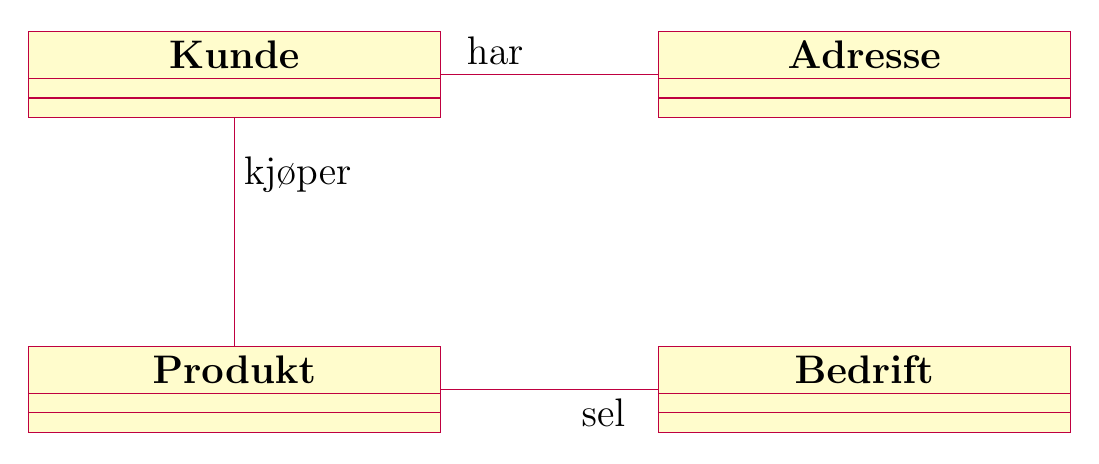
\begin{tikzpicture}
          \tikzstyle{every node}=[font=\Large]

      \begin{class}{Kunde}{0 , 0}
      \end{class}

      \begin{class}{Adresse}{8 , 0}
      \end{class}

      \begin{class}{Produkt}{0, -4}
      \end{class}

      \begin{class}{Bedrift}{8 , -4}
      \end{class}
      \association{Kunde}{kjøper}{}{Produkt}{}{}
      \association{Kunde}{har}{}{Adresse}{}{}
      \association{Bedrift}{sel}{}{Produkt}{}{}


\end{tikzpicture}

\end{document}

       \tikzstyle{every node}=[font=\footnotesize]
